\documentclass{../../../ksp}

\title{KSP 35-H-0}
\author{Daniel Culliver}
\date{Leden 2023}

\begin{document}

\maketitle

\section*{Řešení}

Tady je místo, kde píšeš své brilantní řešení. Text je díky \LaTeX{u} pěkně zarovnaný a díky několika knihovnám i skvěle zvládá češtinu; třeba text v uvozovkách, nebo háčky u \textbf{ť} a \textbf{ď}. Občas se můžou hodit i {\color{red} barvičky}, \underline{podtržení}, nebo \emph{kurzíva}.

Seznamy jsou:

\begin{compactitem}
    \item Kompaktnější
    \item Objektivně estetičtější
\end{compactitem}

Krom toho se hodí umět odkazovat; třeba na \href{https://en.wikibooks.org/wiki/LaTeX/Advanced_Mathematics#Other_environments}{různé způsoby zarovnání matematiky}, na které se podíváme teď. 

\subsection*{Matematika}

Můžeme ji zapisovat v řádku: $e^{ix} = \cos{x} + i \sin{x}$, nebo zarovnaně:
%
\[
    a_0=\frac{1}{\pi}\int\limits_{-\pi}^{\pi}f(x)\,\mathrm{d}x
\]

Krom toho se hodí umět kreslit\footnote{Kreslit je zde samozřejmě použito velmi volně; kreslí za nás počítač. Byla to však skvělá příležitost pro to ukázat poznámku pod čarou.}!

\hfill

% Získáno z https://texample.net/tikz/examples/truncated-cone/
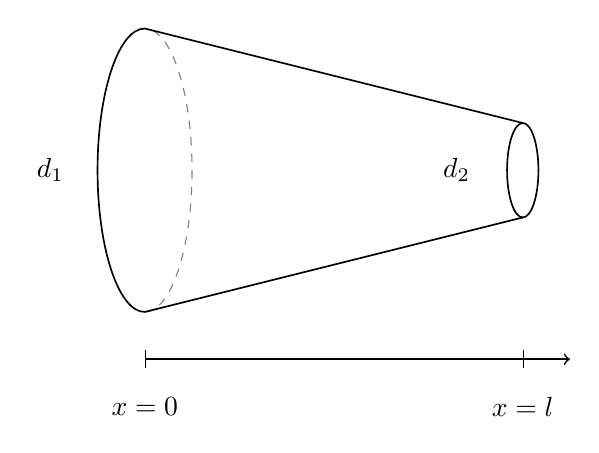
\begin{tikzpicture}[scale=1.2]
    \draw[dashed,color=gray] (0,0) arc (-90:90:0.5 and 1.5);% right half of the left ellipse
    \draw[semithick] (0,0) -- (4,1);% bottom line
    \draw[semithick] (0,3) -- (4,2);% top line
    \draw[semithick] (0,0) arc (270:90:0.5 and 1.5);% left half of the left ellipse
    \draw[semithick] (4,1.5) ellipse (0.166 and 0.5);% right ellipse
    \draw (-1,1.5) node {$\varnothing d_1$};
    \draw (3.3,1.5) node {$\varnothing d_2$};
    \draw[|-,semithick] (0,-0.5) -- (4,-0.5);
    \draw[|->,semithick] (4,-0.5) -- (4.5,-0.5);
    \draw (0,-1) node {$x=0$};
    \draw (4,-1) node {$x=l$};
\end{tikzpicture}

Pro zapisování asymptotické složitosti můžete použít tyhle cool písmenka: $\BigO(n \log n)$

\begin{center}
    {\large Doufám, že se ti tento vzor bude hodit. Hodně štěstí při řešení!}
\end{center}

\end{document}